\chapter{Load Shedding}
\label{ch:load_shedding}

\todo{Intro}

\clearpage
%--------------------------------------------------------------------------------------------------------

\section{Overload Management}

\mnote{A section about shedding. Talk again about how the shedder works, how tuples are dropped.}

\mnote{Also an explanation about "how SIC metrics can be used to reason about the quality of data", so
intelligent shedding.}

\clearpage
%--------------------------------------------------------------------------------------------------------

\subsection{Source Time Window} 

\mnote{How SIC is calculated starting from this.}

\clearpage
%--------------------------------------------------------------------------------------------------------

\subsection{Random Vs Intelligent Shedding}

\clearpage
%--------------------------------------------------------------------------------------------------------

\section{Fair Shedding}
\label{sec:fair-shedding}

\mnote{Fair shedding algorithm description}


\mnote{Random vs Intelligent Evaluation (Figure 8-9-10-11) [let's see how to present these results]}

\clearpage
%--------------------------------------------------------------------------------------------------------

\section{SIC values and query performance}

This section evaluates this correlation across a representative range of \emph{aggregate} and
\emph{top-k} classes of queries. These query types are widely used in a variety of data-processing
applications, such as sensor networks, financial processing, etc. Furthermore, we also include the
calculation of the covariance metric between two time-series data of real numbers which is widely used in
statistics and scientific processing to measure the correlation between two variable.
\innote{stats citation}

\mnote{this text may be moved}
When using the SIC metric to provide feedback on processing quality to users,
it is important that performance of the result of the query output is 
\emph{strictly increasing} to the SIC values: \ie as the SIC values increase,
the query result output is getting \emph{closer} to the perfect result 
without shedding or it does not change. 

\gap
\vskip 5cm

\subsection{Correlation Metrics}

We compare the results of a query with degraded processing---\ie with result
SIC values of less than~1---against the result of a query with perfect
processing. Each query (degraded and perfect) runs for 5~minutes and we measure
the mean error in the results every second as a function of the achieved 
SIC values of the result stream for different data distributions.

For the \textnormal{AVG}, \textnormal{COUNT} and \textnormal{MAX} aggregate 
queries we use the \emph{mean absolute error} that quantifies the relative distance of the
\emph{degraded} from the \emph{perfect} result value across all
measurements~$n$ for the duration of the experiment:
\begin{align}
\frac{ \sum \lvert {\displaystyle \frac{\displaystyle \mathit{degraded} - \displaystyle \mathit{perfect}}{\displaystyle \mathit{perfect}}}  \rvert}{\displaystyle n}
\end{align}

For the \textnormal{TOP-5} query we calculate the error using the
Kendall's distance metric that counts the differences---\ie permutations and
elements in only one list---of pairs of distinct elements between the two
lists~\cite{kendall}. We use the normalised Kendall's distance with a maximum error of 1.

In the case of the \textnormal{COV} we use the following methodology. Each experiment
produces a series of query results; the experiments duration is
5~minutes each and the \textnormal{COV} query outputs a new \emph{sample} 
covariance every 1~sec. These values are random and their expected value 
matched the \emph{real} covariance. 
\innote{stats citation} 
In our case, the real covariance come from perfect processing. Hence, by comparing
the two variables, \ie the degraded sample covariances and the perfect real
covariances, we can evaluate the correlation between the SIC values and the 
\textnormal{COV} query results. We compare the two variables through their
standard deviations.  



\subsection{Experimental Setup}

For the current evaluation the Local test-bed is used. We overload a single 
\sys node by instantiating an increasing number of queries of a single type of 
queries listed in Table~\ref{table:queries}. 
As we increase the number of queries, the node discards an increasing number 
of tuples. The node uses a tuple shedder that sheds tuples randomly from each query.
We repeat the experiment for every query type and across five different 
sets of source data. The shedding interval is set to 250~milliseconds.

Throughout the experimental evaluation, we deploy queries that belong to one
of the following two mixes: aggregate (\ie \textnormal{AVG}, \textnormal{MAX}
and \textnormal{COUNT}) and complex (\ie \textnormal{TOP-5}), \textnormal{AVG-all} and 
\textnormal{COV1}) queries; they are
summarised in Table~\ref{table:queries}. The queries use a diverse set of
operators, namely: \textnormal{average}, \textnormal{max}, \textnormal{top-k}, 
\textnormal{group-by}, \textnormal{filter}, \textnormal{join}, \textnormal{cov}, 
\textnormal{time-window}, \textnormal{remote-sender}, \textnormal{remote-receiver} 
and \textnormal{output}.

We use various data sources that produce streams with synthetic or real-world
data at various rates. The values of the synthetic data follow either a
\emph{gaussian}, \emph{uniform} or \emph{exponential} distribution that
have a mean of 50. We also support an \emph{advanced} synthetic workload that mixes all three
distributions randomly. The real-world data streams are traces from CPU load and memory
usage measurements from all PlanetLab nodes~\cite{planetlab} in April~2010, as
recorded by the CoTop project~\cite{cotop}. 
Sources generate data streams at various rates as will be reported throughout 
the evaluation. 

In all experiments, we set the duration of the source time window~(STW) for all
sources to 10~secs. This value stays well within the variation of processing
delays across evaluation queries.
 
%% --- TABLE TESTBED ---

%% --- TABLE TESTBED ----
\begin{table}[b!]
  %\centering
  \hspace{0.8cm}
  \renewcommand{\arraystretch}{1.5}
  \begin{tabular}{|m{3cm}|p{12cm}|} 
  \hline
  \multicolumn{2}{|c|}{\bf Local Testbed} \\ 
  
    \hline\hline
	Physical configuration
	& 
	3 machines with 1.8~Ghz CPUs and 4~GB of memory running Ubuntu Linux 2.6.27-17-server and connected
	over 1~Gbps network. \\
    \hline
	
	System layout
	&
	1 machine: oracle node; 1 machine: source data generation and query submission; 1 machine: \sys
	processing node. \\
    \hline
	
	Data sources
	&
	400~tuples/sec in 5~batches/sec of 80~tuples/batch. 
	\\
    \hline\hline
    
    \multicolumn{2}{|c|}{\bf Emulab Testbed} \\ 
    \hline\hline
	Physical layout
	&	
	pc3000-type machines connected over a 1~Gbps LAN network. Each machine has a 3~Ghz CPU, 2~GB of
	memory and runs the FBSD410+RHL90-STD Emulab-configured Linux image.
	\\
    \hline
	System layout
	&
	1 machine: 1 oracle node;
	3 machines: source data generation; 
	3 machines: query submission;
	18 machines: 18 \sys processing nodes. \\
    \hline
	
	Data sources
	& 
	150~tuples/sec in 3~batches/sec of 50~tuples/batch. \\
	
    \hline\hline 
  \end{tabular}
  \caption{Testbed configurations for experiments. }
  \label{table:machines}
\end{table}


%% --- TABLE QUERIES ---
%% --- TABLE QU1ERIES ---
\begin{table}[h!]
  \centering
  \renewcommand{\arraystretch}{1.5}
  \begin{tabular}{|m{3cm}|p{12cm}|}
    \hline
    \multicolumn{2}{|c|}{\bf Aggregate Queries} \\ 
    \hline\hline
    \textnormal{AVG}	&  Calculates the average value over 1~sec. \\ 
%     \hline
%     \textnormal{MAX}	&  Calculates the maximum value over 1~sec. \\ 
    \hline	  
    \textnormal{COUNT}	&  Counts the number of tuples with values $>=$ 50.0 over 1~sec.  \\  
    \hline\hline
    \multicolumn{2}{|c|}{\bf Complex Queries} \\ 
    \hline \hline
    \textnormal{TOP-5}	&  Shows the 5~PlanetLab nodes with the
    highest amount of available CPU and at least 100~KB of free memory over 1~sec.\\
    \hline	  
%     \textnormal{AVG-all} & Shows the avg CPU consumption over
%     PlanetLab nodes over 1~sec. \\
%     \hline	  
    \textnormal{COV} &  Shows the covariance of the CPU cycles consumption between two PlanetLab nodes.
    \\
    \hline	  
  \end{tabular}
  \caption{Query workload for experiments.}
  \label{table:queries}
\end{table}


The \textnormal{AVG}, \textnormal{COUNT} and \textnormal{MAX}
aggregate queries connect to one source with a rate of 400~tuples/sec and \textnormal{COV}
queries connect to two sources of 400~tuples/sec. 
The \textnormal{TOP-5} query connects to 20~sources, equally split between CPU load and
memory readings. Each source has a rate of 20~tuples/sec. To create a skewed
distribution for the \textnormal{TOP-5} query, the mean for 10~sources is increased
from 50 to 230 in steps of 20.


\clearpage
%--------------------------------------------------------------------------------------------------------

\subsection{Aggregate Queries}

\mnote{Simple queries: AVG, COUNT, MAX queries (Figure 5: Correlation of the SIC values with the query
output performance, aggregate queries)}
 
For the \textnormal{AVG} query (Figure~\ref{fig:agg-avg}), the result has a small error
after shedding because the average of the new distribution does not change
significantly. For the \textnormal{COUNT} query in Figure~\ref{fig:agg-count}, however,
there is a linear correlation. In the case of the \textnormal{MAX} query, we note
the result has a small error for the synthetic distributions. However, the error
increases and shows a linear correlation in the case of the mixed and the PlanetLab
distributions. Overall, the more source tuples are used for a result
stream, the more accurate the result output is.

% ---- AVG FIGURE -----
\begin{figure*}[h]
\centering
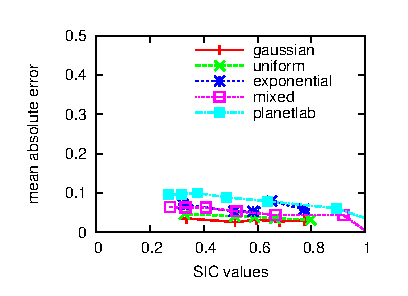
\includegraphics[width=0.6\textwidth]{img/tesi/avg1}
\caption{Aggregate \emph{Average} queries, correlation of SIC values with the query output performance.}
\label{fig:agg-avg}
\end{figure*} 

% ---- COUNT FIGURE -----
\begin{figure*}[h]
\centering
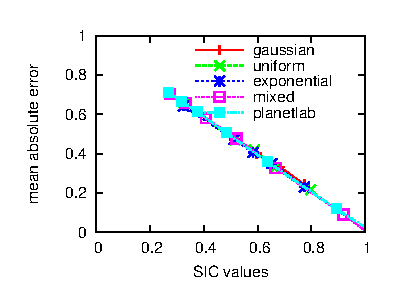
\includegraphics[width=0.6\textwidth]{img/tesi/count1}
\caption{Aggregate \emph{Count} queries, correlation of SIC values with the query output performance.}
\label{fig:agg-count}
\end{figure*}

% ---- MAX FIGURE -----
\begin{figure*}[t]
\centering
\label{fig:max}
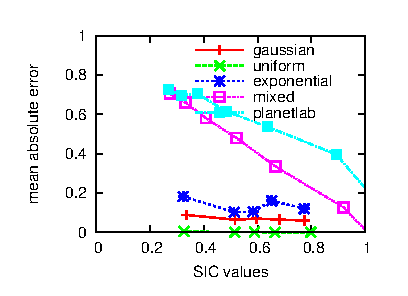
\includegraphics[width=0.6\textwidth]{img/tesi/max1}
\caption{Aggregate \emph{Max} queries, correlation of SIC values with the query output performance.}
\label{fig:agg-max}
\end{figure*}

\clearpage
%--------------------------------------------------------------------------------------------------------


\subsection{Complex Queries}

\mnote{Complex queries:TOP-5, COV}

For the more complicated \textnormal{TOP-5} query in Figure~\ref{fig:top5}, the 
error in the result decreases with the number of source tuples processed. For the
\textnormal{COV} query in Figure~\ref{fig:cov} the std of the result covariances
decreases and approaches the perfect result, \ie SIC $\rightarrow$ 1, as less source data are shed and the
SIC values increase. 

The results show that there in most cases there is a strictly increasing 
correlation between the result SIC values and the distance/error to the perfect result: 
the more the SIC values increase, the smaller the error. The degree of correlation 
depends on the type of query and the source data
distribution. When tuples are discarded randomly, tuples with values across the
range of the initial distributions are chosen at random. The distribution of
the values of admitted tuples are correlated with the original distribution.

% ---- COVARIANCE FIGURE -----
\begin{figure}[h]
\centering
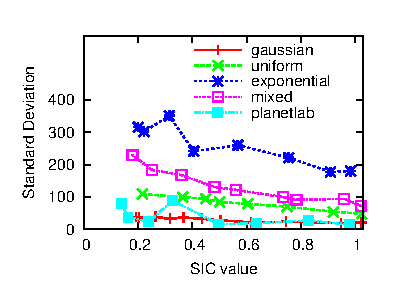
\includegraphics[width=0.6\textwidth]{img/tesi/cov}
\caption{Correlation of the SIC values with the query output performance, \emph{covariance} queries.}
\label{fig:cov}
\end{figure}

% ---- TOP-K FIGURE -----
\begin{figure}[h]
\centering 
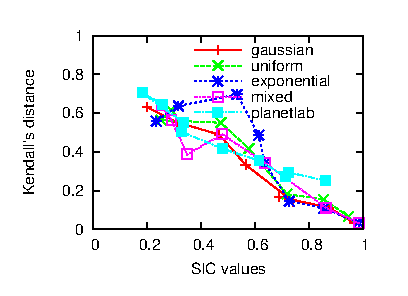
\includegraphics[width=0.6\textwidth]{img/tesi/topK-distance}
\caption{Correlation of the SIC values with the query output performance, \emph{top-k} queries.}
\label{fig:top5}
\end{figure}

